\documentclass[tikz,border=5mm]{standalone}
\usepackage{amsmath,amssymb}
\usepackage{fontspec}

\usetikzlibrary{positioning,arrows.meta,shapes.geometric,fit,backgrounds}

% Master Academic Palette (WCAG AA & Color-Vision Deficiency Compliant)
\definecolor{navyblue}{RGB}{30, 60, 105}    % #1E3C69 - Model architectures, encoders, primary flows
\definecolor{tealblue}{RGB}{20, 110, 105}   % #146E69 - Data plane, ingestion, datasets, gold annotations
\definecolor{purplecat}{RGB}{95, 45, 120}   % #5F2D78 - Multi-task balancing, loss dynamics, statistics
\definecolor{ambergold}{RGB}{180, 85, 15}   % #B4550F - Hardware testbed, serving trials, embeddings
\definecolor{forestgreen}{RGB}{25, 115, 60} % #19733C - Acceptance gates, verified thresholds
\definecolor{crimsonred}{RGB}{175, 40, 40}  % #AF2828 - Feedback loops, out-of-domain holdouts, errors
\definecolor{slategrey}{RGB}{70, 85, 100}   % #465564 - Neutral boundaries, containers, baseline nodes

\begin{document}
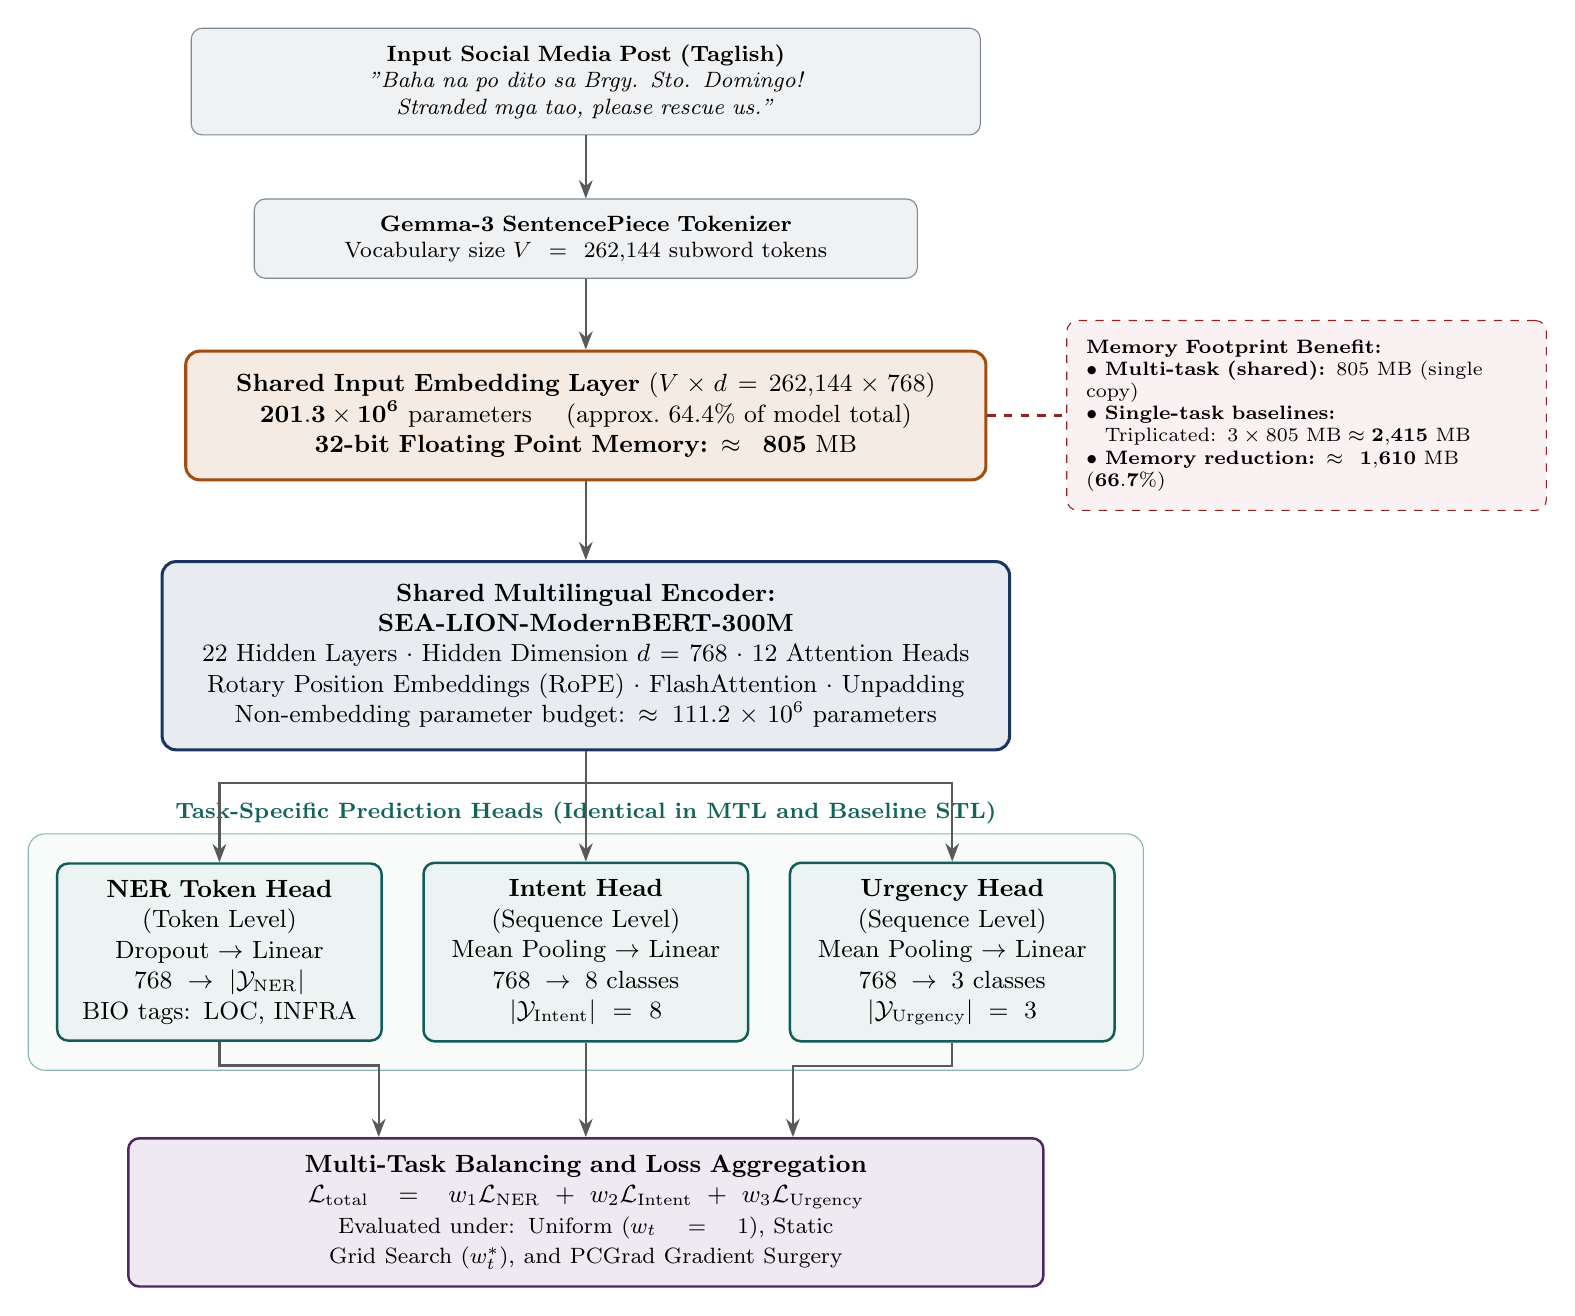
\begin{tikzpicture}[
    font=\small,
    >=Stealth,
    node distance=1.1cm and 0.5cm,
    io/.style={
        draw=slategrey!70,
        fill=slategrey!8,
        rounded corners=4pt,
        align=center,
        inner sep=6pt,
        font=\footnotesize
    },
    embed/.style={
        draw=ambergold!90!black,
        fill=ambergold!12,
        rounded corners=5pt,
        align=center,
        inner sep=8pt,
        line width=1.1pt
    },
    encoder/.style={
        draw=navyblue!90!black,
        fill=navyblue!10,
        rounded corners=5pt,
        align=center,
        inner sep=8pt,
        line width=1.1pt
    },
    head/.style={
        draw=tealblue!85!black,
        fill=tealblue!8,
        rounded corners=4pt,
        align=center,
        inner sep=6pt,
        line width=0.9pt
    },
    loss/.style={
        draw=purplecat!85!black,
        fill=purplecat!10,
        rounded corners=4pt,
        align=center,
        inner sep=6pt,
        line width=0.9pt
    },
    callout/.style={
        draw=crimsonred!85!black,
        fill=crimsonred!6,
        dashed,
        rounded corners=4pt,
        align=left,
        inner sep=7pt,
        font=\scriptsize
    },
    arrow/.style={
        ->,
        thick,
        draw=gray!70!black
    }
]

    % 1. Input and Tokenizer
    \node[io, text width=9.6cm] (input) {
        \textbf{Input Social Media Post (Taglish)}\\
        \textit{"Baha na po dito sa Brgy. Sto. Domingo! Stranded mga tao, please rescue us."}
    };

    \node[io, below=0.8cm of input, text width=8.0cm] (tok) {
        \textbf{Gemma-3 SentencePiece Tokenizer}\\
        Vocabulary size $V = 262{,}144$ subword tokens
    };

    % 2. Input Embedding Matrix (Memory Bottleneck)
    \node[embed, below=0.9cm of tok, text width=9.6cm] (emb) {
        \textbf{Shared Input Embedding Layer} ($V \times d = 262{,}144 \times 768$)\\
        $\mathbf{201.3 \times 10^6 \text{ parameters}}$ \quad (approx.\ $64.4\%$ of model total)\\
        \textbf{32-bit Floating Point Memory:} $\approx \mathbf{805\text{ MB}}$
    };

    % Callout for parameter triplication contrast
    \node[callout, right=1.0cm of emb, text width=5.6cm] (memcall) {
        \textbf{Memory Footprint Benefit:}\\
        $\bullet$ \textbf{Multi-task (shared):} $805\text{ MB}$ (single copy)\\
        $\bullet$ \textbf{Single-task baselines:}\\
        \phantom{$\bullet$} Triplicated: $3 \times 805\text{ MB} \approx \mathbf{2{,}415\text{ MB}}$\\
        $\bullet$ \textbf{Memory reduction:} $\approx \mathbf{1{,}610\text{ MB}}$ ($\mathbf{66.7\%}$)
    };

    % 3. Shared Encoder Stack
    \node[encoder, below=1.0cm of emb, text width=10.2cm] (enc) {
        \textbf{Shared Multilingual Encoder: SEA-LION-ModernBERT-300M}\\
        22 Hidden Layers $\cdot$ Hidden Dimension $d = 768$ $\cdot$ 12 Attention Heads\\
        Rotary Position Embeddings (RoPE) $\cdot$ FlashAttention $\cdot$ Unpadding\\
        Non-embedding parameter budget: $\approx 111.2 \times 10^6 \text{ parameters}$
    };

    % 4. Task Prediction Heads
    \node[head, below=1.4cm of enc, text width=3.7cm] (intent) {
        \textbf{Intent Head}\\
        (Sequence Level)\\
        Mean Pooling $\to$ Linear\\
        $768 \to 8 \text{ classes}$\\
        $|\mathcal{Y}_{\text{Intent}}| = 8$
    };

    \node[head, left=0.5cm of intent, text width=3.7cm] (ner) {
        \textbf{NER Token Head}\\
        (Token Level)\\
        Dropout $\to$ Linear\\
        $768 \to |\mathcal{Y}_{\text{NER}}|$\\
        BIO tags: LOC, INFRA
    };

    \node[head, right=0.5cm of intent, text width=3.7cm] (urgency) {
        \textbf{Urgency Head}\\
        (Sequence Level)\\
        Mean Pooling $\to$ Linear\\
        $768 \to 3 \text{ classes}$\\
        $|\mathcal{Y}_{\text{Urgency}}| = 3$
    };

    % Task head container background
    \begin{scope}[on background layer]
        \node[draw=tealblue!50, fill=tealblue!3, rounded corners=6pt, fit=(ner) (intent) (urgency), inner sep=10pt, label={[tealblue!90!black, font=\footnotesize\bfseries]above:Task-Specific Prediction Heads (Identical in MTL and Baseline STL)}] (headsbox) {};
    \end{scope}

    % 5. Loss Aggregation and Balancing
    \node[loss, below=1.2cm of intent, text width=11.2cm] (lossbox) {
        \textbf{Multi-Task Balancing and Loss Aggregation}\\
        $\mathcal{L}_{\text{total}} = w_1 \mathcal{L}_{\text{NER}} + w_2 \mathcal{L}_{\text{Intent}} + w_3 \mathcal{L}_{\text{Urgency}}$\\
        \footnotesize Evaluated under: Uniform ($w_t = 1$), Static Grid Search ($w_t^*$), and PCGrad Gradient Surgery
    };

    % Connections
    \draw[arrow] (input) -- (tok);
    \draw[arrow] (tok) -- (emb);
    \draw[arrow] (emb) -- (enc);
    \draw[dashed, crimsonred!85!black, thick] (emb.east) -- (memcall.west);

    % Encoder to Heads
    \draw[arrow] (enc.south) -- ++(0,-0.4) -| (ner.north);
    \draw[arrow] (enc.south) -- (intent.north);
    \draw[arrow] (enc.south) -- ++(0,-0.4) -| (urgency.north);

    % Heads to Loss
    \draw[arrow] (ner.south) |- ++(0,-0.3) -| (lossbox.160);
    \draw[arrow] (intent.south) -- (lossbox.north);
    \draw[arrow] (urgency.south) |- ++(0,-0.3) -| (lossbox.20);

\end{tikzpicture}
\end{document}
